\newpage
\setcounter{figure}{0}

\section{Pregled korištenih tehnologija i algoritama} % (fold)
\label{sec:Tehnologija i teorija}


\subsection{Microsof Kinect 3D kamera} % (fold)
\label{sub:Microsof Kinect 3D kamera}

% subsection Microsof Kinect 3D kamera (end)

\subsection{ROS biblioteka i alati} % (fold)
\label{sub:ROS biblioteka i alati}

% subsection ROS biblioteka i alati (end)

\subsection{Biblioteka Pointcloud} % (fold)
\label{sub:Biblioteka Pointcloud}

% subsection Biblioteka Pointcloud (end)


\newpage
\subsection{Istovremena lokalizacija i mapiranje} % (fold)
\label{sub:Slam}
Istovremena lokalizacija i mapiranje dolazi od engleske skraćenice
SLAM \textit{Simultaneous Localization and Mapping}. SLAM su
originalno razvili Hugh Durrant-Whyte i John J.
Leonard~\cite{Durrant:91b} koji su rad bazirali na prethodnom radu
Smitha, Selfa and Cheesemana~\cite{Smith86}. SLAM se bavi rješavanjem
problema izgradnje mape nepoznate okoline mobilnog robota te istovremeno
navigiranje robota okolinom koristeći tu mapu.

SLAM se sastoji iz nekoliko koraka: izvlačenje orijentira, asociranje
podataka, estimiranja stanja, ažuriranja stanja i ažuriranja orijentira.
Postoji više načina kako riješiti svaki od tih koraka. SLAM se može
primjeniti na 2D i 3D kretanje.

\subsubsection{Osnovna ideja i kratak pregled koraka} % (fold)
\label{ssub:Osnovna ideja }
Proces istovremene lokalizacije i mapiranja se sastoji iz nekoliko
koraka. Cilj procesa je koristiti okolinu za ažuriranje pozicije robota.
Zbog nesavršenosti odometrije robota nije dobro osloniti se samo na nju
kako bi se pronašla pozicija robota. Već se može koristiti lasersko
skeniranje okoline ili kao u slučaju RGBDSlam programa Kinect 3D kamera
kako bi pronašli pravu poziciju robota/kamere. To se postiže
izvlačenjem značjaki iz okoline i promatranjem tih značajki kada se
robot pomakne. EKF (\textit{Extended Kalman Filter}) prošireni Kalmanov
filter je jezgra SLAM procesa. EKF je odgovoran za ažuriranje pozicije
na kojoj robot misli da se nalazi koristeći izvučene značajke. Takve
značajke se još nazivaju i orjentiri. EKF prati estimaciju nesigurnosti
pozicije robota i nesigurnosti orijentira iz okoline. Pregled SLAM
procesa~\footnotemark[1] se nalazi na grafikonu~\ref{fig:slam-overview.pdf}  

\begin{figure}[h]
\renewcommand{\figurename}{Grafikon}
\centering
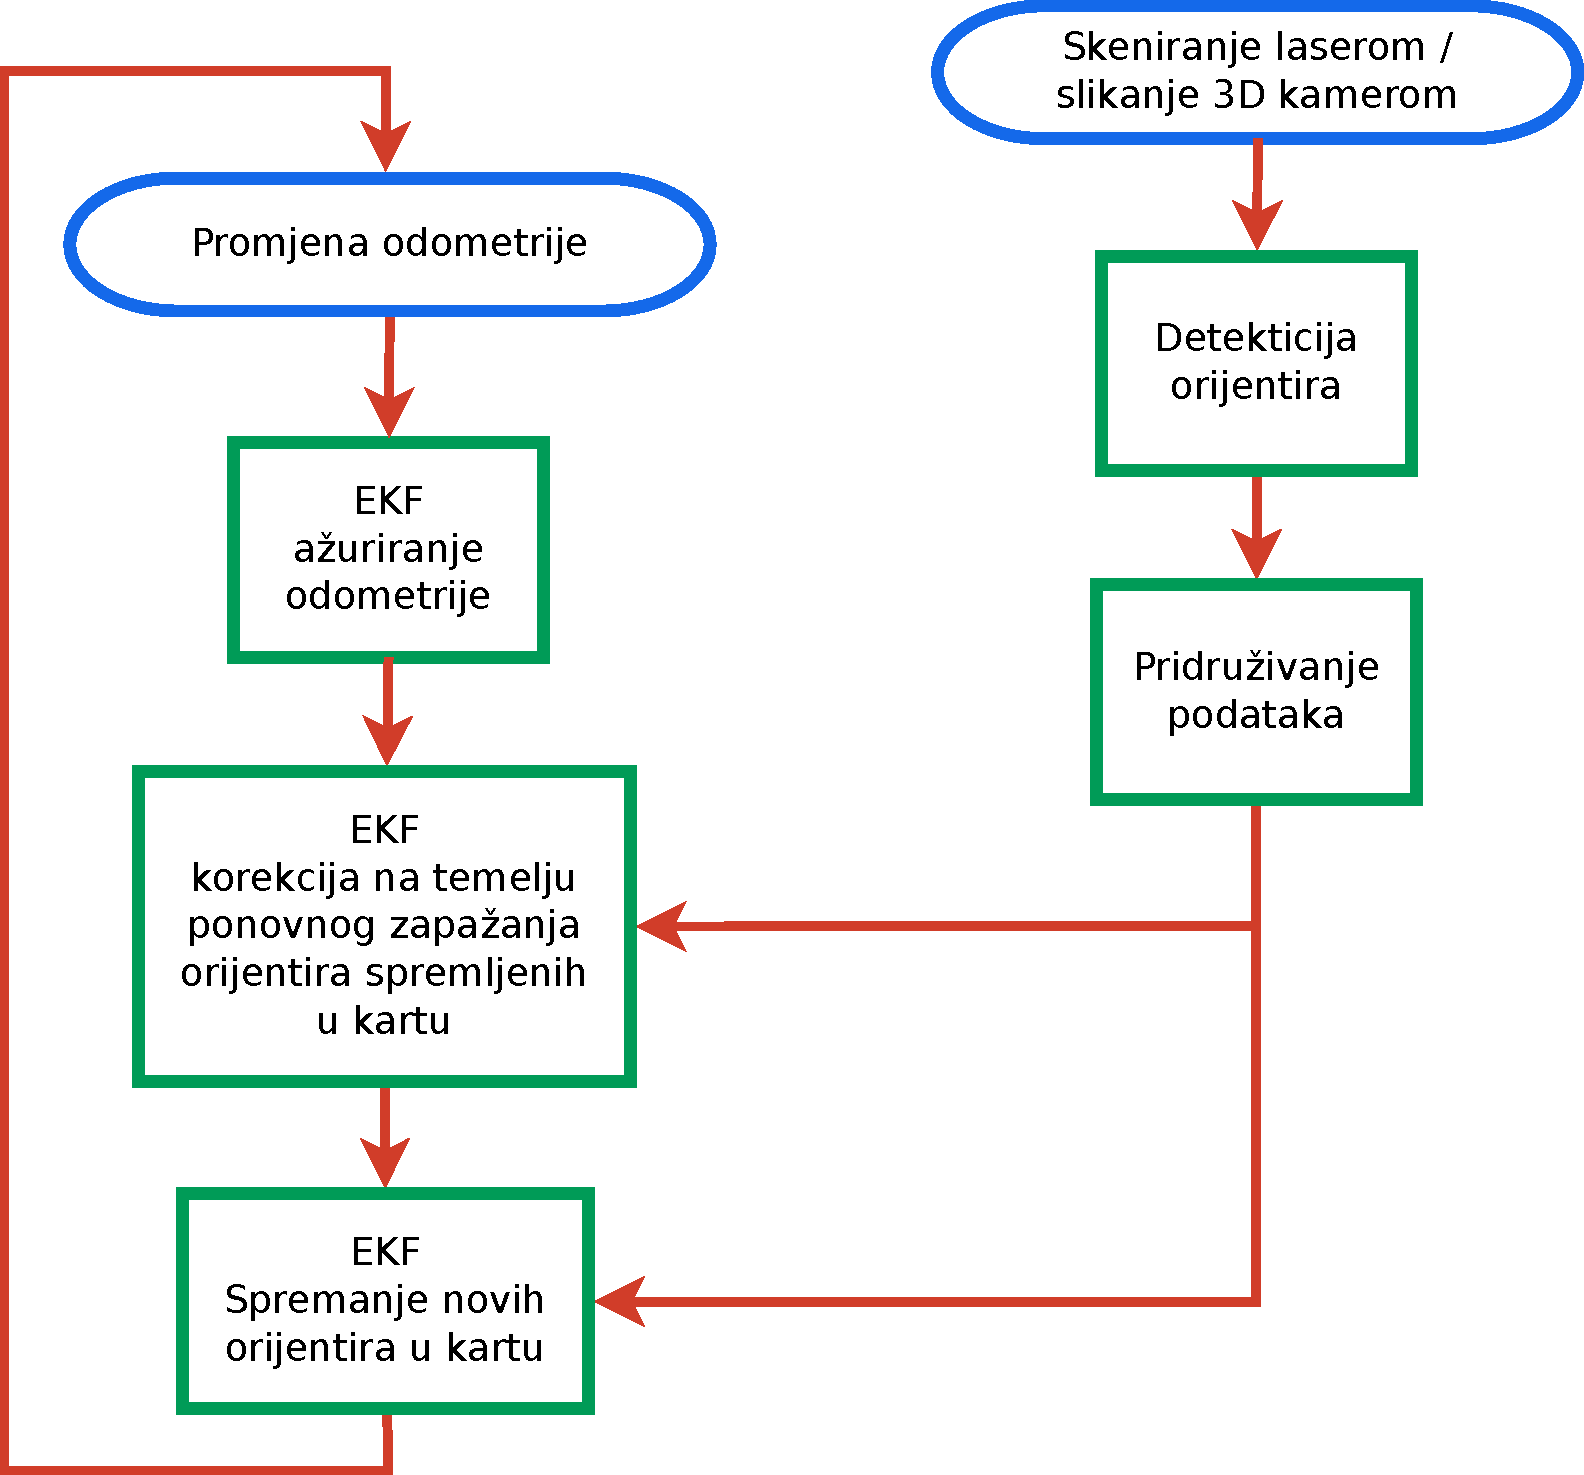
\includegraphics[scale=0.43]{figures/slam-overview.pdf}
\caption{Pregled SLAM procesa}
\label{fig:slam-overview.pdf}
\end{figure}

Kad se odometrija promjeni zato što se robot pomakao nesigurnost koja se
tiče robotove nove pozicije se ažurira u EKF koristeći ažuriranje
odometrije. Orijentiri se tada izvlače iz okoline zbog robotove nove
pozicije. Robot tada pokušava asocirati te orijentire s prije pronađenim
orijentirima. Ponovno pronađeni orijentiri se tada koriste za ažuriranje
pozicije robota u EKFu. Orijentiri koji prije nisu pronađeni se dodaju u
EKF kako bih se mogli koristiti kasnije. U svakom od opisanih koraka EKF
računa estimaciju robotove trenutne pozicije.

\footnotetext[1]{%
Grafikon je inspiriran sličnim grafikonom iz rada SLAM for
Dummies~\cite{web:slam} }

% subsubsection Osnovna ideja  (end)
% subsection Slam (end)

\newpage
\subsection{Poisson algoritam za rekonstrukciju površine} % (fold)
\label{sub:Poisson}
Poisson algoritam za rekonstrukciju površine~\cite{Kazhdan:2006}
razvijen je suradnjom Michaela Kazhdana i Matthewa Bolitha s Johns
Hopkins sveučilišta u Baltimoru i Huguesa Hoppea iz Microsoft Researcha
u Redmondu. Također Kazhdan i Bolitho su implementirali\footnotemark[1]
Poisson algoritam i objavili kod pod BSD licencom. Na osnovu tog rada
algoritam je dodan i u PCL biblioteku.

U ovom potpoglavlju nalazi se osnovna ideja i kratak matematički pregled
algoritma. Opisano je ograničenje algoritma te parametri kojima se može
upravljati rekonstrukcijom površine.

\footnotetext[1]{%
Originalna implementacija Poisson algoritma se nalazi na 
\url{http://www.cs.jhu.edu/~misha/Code/PoissonRecon/Version5.5/}}

% Rekonstrukcija 3D površina iz uzorka točaka je dobro proučavan problem u
% računalnoj grafici. Ona omogućava uklapanje skeniranih
% podataka, ispunjavanje površinskih rupa i ponovnu izgradnju postojećih
% modela.

\subsubsection{Osnovna ideja i kratak matematički pregled} % (fold)
\label{ssub:Osnovna ideja i kratak matematički pregled}

Poisson algoritam pristupa problemu rekonstrukcije površine rješavanjem
Poissonove jednadžbe. To čini upotrebom metode implicitne funkcije.
Točnije računanjem 3D indikacijske funkcije \(\chi\) definirane s 1 u
točkama unutar modela, odnosno s 0 u točkama izvan i dohvaćanjem
rekonstruktruirane površine izvlačenjem odgovarajuće izopovršine.

Algoritam se oslanja na ideju da postoji cjelovita veza između
orijentiranih normala uzetih s površine modela i indikacijske funkcije
modela. Točnije, gradijent indikacijske funkcije je polje vektora koje
je uglavnom popunjeno nulama (jer je indikacijska funkcija uglavnom
konstantna), osim kod točaka blizu površine gdje je jednako unutrašnjim
normalama površine. Stoga, uzorci orijentiranih normala mogu biti
promatrani kao gradijent modela indikacijske funkcije kao što je
prikazano na slici~\ref{fig:poisson-reconstruction.png}

\begin{figure}[h]
\centering
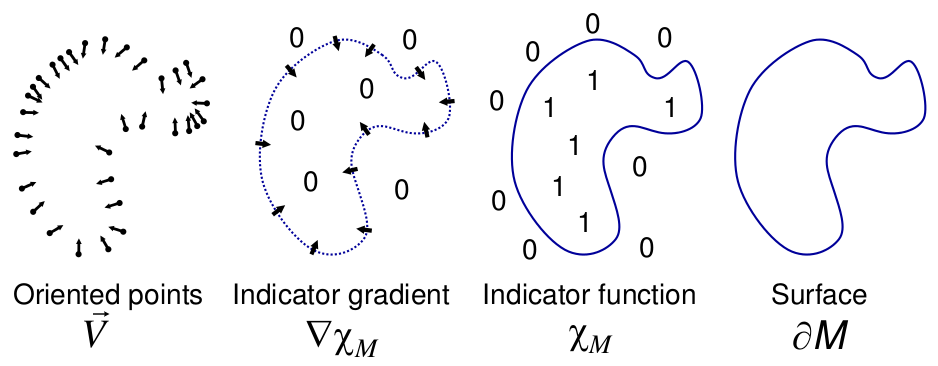
\includegraphics[scale=0.35]{figures/poisson-reconstruction.png}
\caption[]{Prikaz Poisson rekonstrukcije u 2D,
    izvor:~\cite{Kazhdan:2006}}
\label{fig:poisson-reconstruction.png}
\end{figure}

Problem računanja indikacijske funkcije se svodi na invertiranje
operatora gradijenta, odnosno pronalazak funkcije skalara \(\chi\) čiji
gradijent najbolje aproksimira polje vektora \(\vec{V}\) definirano
uzorcima, odnosno 

\begin{equation*}
min_\chi \|\nabla\chi - \vec{V}\|.
\end{equation*}

Ako se primjeni operator divergencije, tada se taj problem pretvara u
standardni Poissonov problem: računanje funkcije skalara \(\chi\) čiji
laplasijan (divergencija gradijenta) je jednak divergenciji polja
vektora \(\vec{V}\),

\begin{equation*}
\Delta \chi \equiv \nabla \cdot \nabla\chi = \nabla \cdot \vec{V}.
\end{equation*}

Predstavljanje rekonstrukciju površine kao Poissonov problem pruža
nekoliko prednosti. Mnoge implicitne metode uklapanja površina
segementiraju podatke u regije za lokalno uklapanje i onda te lokalne
aproksimacije spajaju upotrebom funkcija stapanja. Za razliku od njih,
Poisson rekonstrukcija je globalno rješenje koje razmatra sve podatke
odjednom, bez upotrebe heurstičkih podijela i stapanja. Zbog toga
Poisson rekonstrukcija kreira izrazito glatku površinu koja robusno
aproksimira šumovite podatke.  

Za izvlačenje izopovršine Poisson algoritam koristi Marching Cubes
algoritam~\cite{Lorensen87marchingcubes} koji kreira octree strukturu
podataka za prikaz površine.  Kao što se vidi na
slici~\ref{fig:poisson-marching-cubes.png} Marching Cubes algoritam
dijeli oblak točaka u mrežu voxela marširajući kroz oblak i analizira
koje točke čine izopovršinu objekta.  Detektiranjem koji rubovi voxela
presjecaju izopovršinu modela algoritam kreira mrežu trokuta. Više
informacija o izvlačenju površine se mogu pronaći u radu “Unconstrained
Isosurface Extraction on Arbitrary Octrees” Michaela
Kahzdana~\cite{Kazhdan:2007}

\begin{figure}[h]
\centering
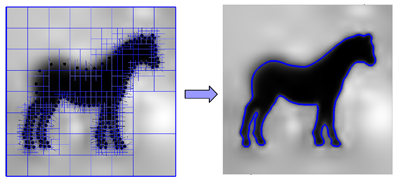
\includegraphics[scale=0.8]{figures/poisson-marching-cubes.png}
\caption[]{Prikaz Marching cubes algoritma, izvor:~\cite{Kazhdan:2007}}
\label{fig:poisson-marching-cubes.png}
\end{figure}

% subsubsection Osnovna ideja i kratak matematički pregled (end)

\subsubsection{Ograničenje Poisson algoritma} % (fold)
\label{ssub:Ograničenje Poisson algoritma}

Ograničenje implementacije Poisson algoritma je u tome što ne uzima u
obzir informacije asocirane s načinom stjecanja oblaka točaka.
Slika~\ref{fig:poisson-buddha.png} pokazuje kip Bude i vidi se primjer takvog
ograničenja. Budući da nema točaka između Budinih nogu, Poisson
algoritam spaja te dvije regije. Algoritam se može unaprijediti
ugradnjom dodatne informacije poput vidokruga i na taj način izbjeći to
ograničenje.

**A limitation of our method
is that it does not incorporate information associated with
the acquisition modality. Figure 6 shows an example of this
in the reconstruction at the base of the Buddha. Since there
are no samples between the two feet, our method (right)
connects the two regions. In contrast, the ability to use sec-
ondary information such as line of sight allows VRIP (left)
to perform the space carving necessary to disconnect the two
feet, resulting in a more accurate reconstruction.**


\begin{figure}[h]
\centering
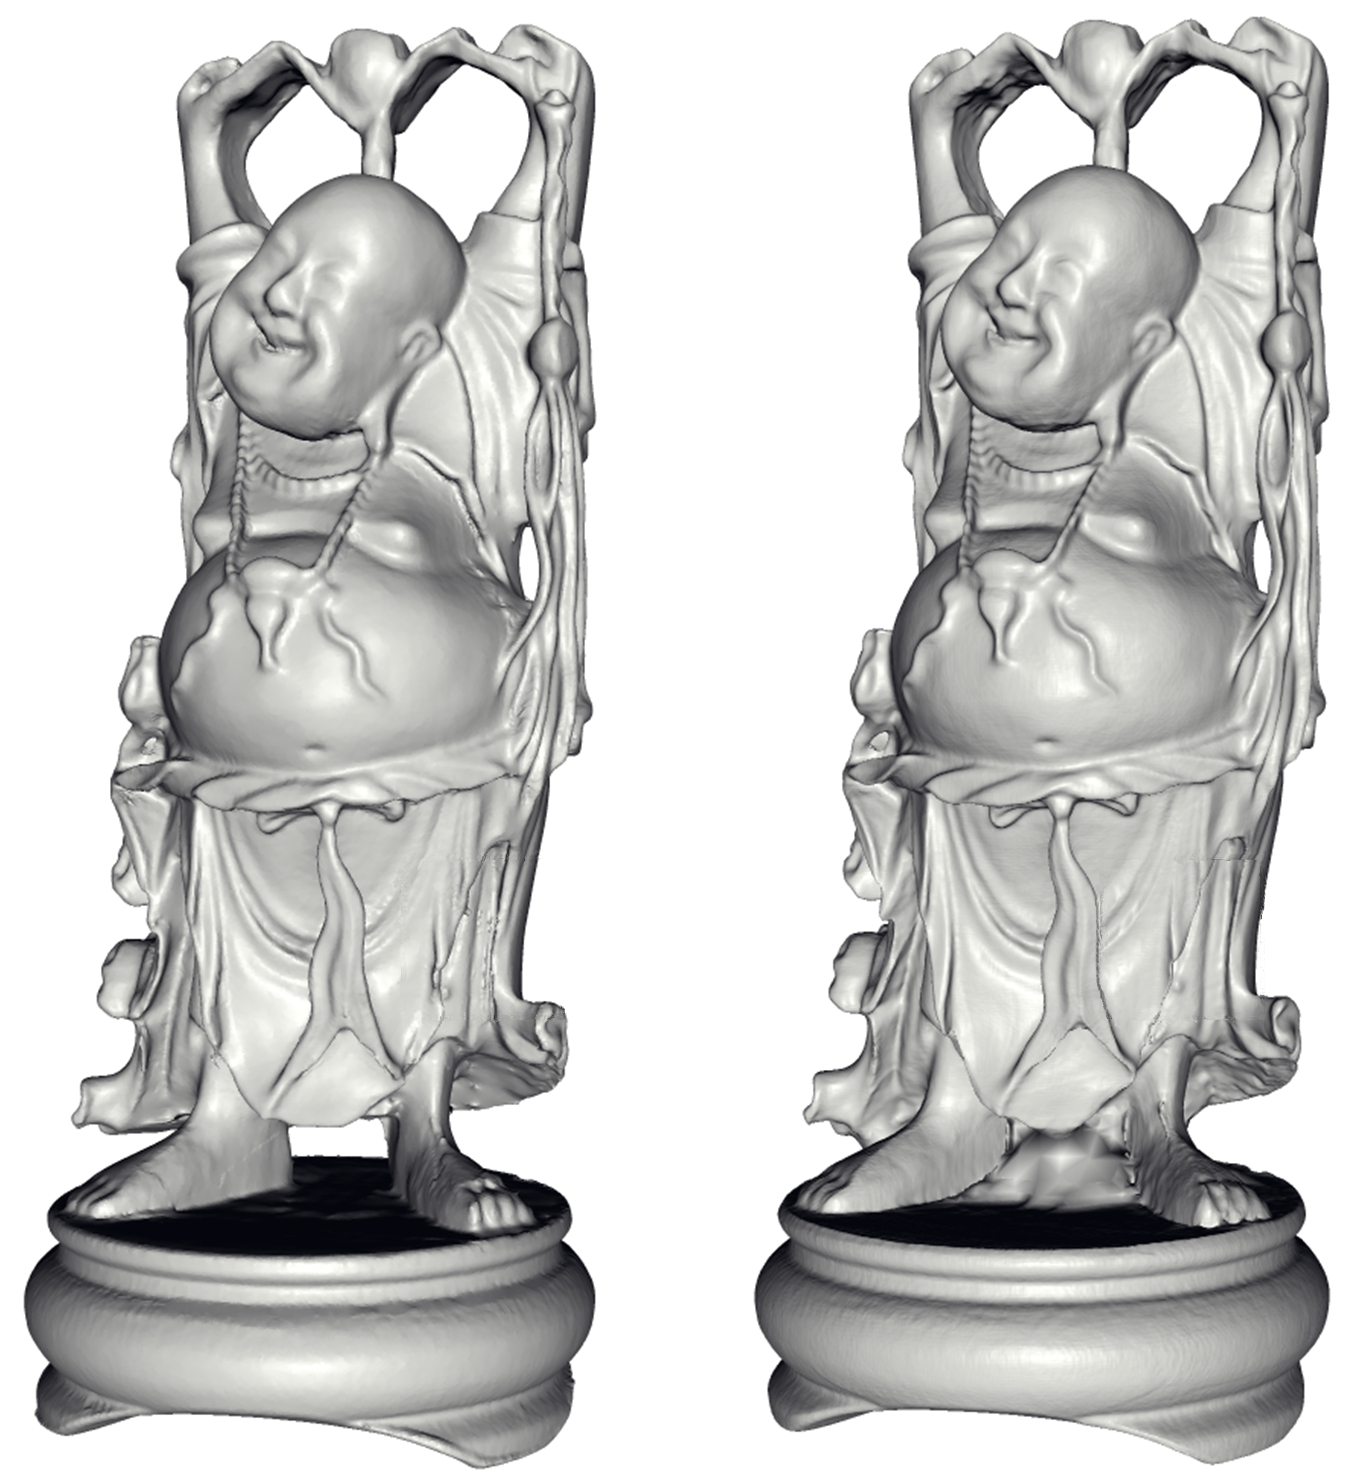
\includegraphics[scale=0.20]{figures/poisson-buddha.png}
\caption[]{Rekonstrukcija modela ``Happy Buddha'' 
VRIP\footnotemark[2] algoritam (lijevo) i Poisson algoritma (desno),
izvor:~\cite{Kazhdan:2006}}
\label{fig:poisson-buddha.png}
\end{figure}

\footnotetext[2]{%
VRIP - Volumetric Range Image Processing~\cite{Curless:1996VRIP}}

% subsubsection Ograničenje Poisson algoritma (end)

\newpage
\subsubsection{Parametri Poisson algoritma} % (fold)
\label{ssub:Parametri Poisson algoritma}
Postoji nekoliko parametara koji utječu na rezultat rekonstrukcije.
\begin{itemize}
    \item \texttt{Depth:} dubina octree stabla koje se koristi za
        rekonstrukciju. Pretpostavljena vrijednost 8.
    \item \texttt{SolverDivide:} postavlja dubinu kod kojeg bloka
        Gauss-Seidel metoda riješava Laplaceovu jednadžbu. Pretpostavljena
        vrijednost 8.
    \item \texttt{IsoDivide:} postavlja dubinu kod kojeg bloka
        ekstraktor izopovršine izvlači izopovršinu. Pretpostavljena vrijednost
        8.
    \item \texttt{SamplesPerNode:} postavlja minimalni broj točaka koje
        se trebaju nalaziti unutar octree čvora kako se octree
        konstrukcija prilagođava gustoći uzorkovanja. Za podatke bez
        šuma 1 - 5, sa šumom 15 - 20. Pretpostavljena vrijednost 1.
    \item \texttt{Scale:} omjer između promjera kocke korištne za
        rekonstrukciju i promjera kocke koja omeđuje uzorke. Pretpostavljena
        vrijednost 1.25.
    \item \texttt{Confidence:} postavljanje zastavice govori
        rekonstruktorciji da koristi veličinu normala kao informaciju o
        pouzdanosti. Ako nije postavljena sve normale se normaliziraju
        prije rekonstrukcije.
\end{itemize}

Od nabrojanih parametara najvažniji utjecaj na generiranu mrežu imaju
\texttt{SamplesPerNode} i \texttt{Depth}. Veća dubina octree stabla
rezultira većom precinosti mreže voxela jer Marching Cubes algoritam
ulazi dublje u stablo. Manja dubina (između 5 i 7) daje glađi model ali
s manje detalja. \texttt{SamplesPerNode} parametar definira koliko će
točaka Marchin Cubes algoritma staviti u jedan čvor rezultantnog octree
stabla. Ako algoritam radi s podacima punim šuma velik uzorak točaka (15
- 20) po čvoru pruža glađenje ali se gube detalji. Dok rad s malim
vrijednostima (1 - 5) održava razinu detalja visokom. Velike vrijednosti
reduciraju kranji broj vrhova poligona, dok male održavaju broj vrhova
visokim.

% subsubsection Parametri Poisson algoritma (end)

% subsection Poisson (end)

% section Tehnologija i teorija (end)
